% SPDX-FileCopyrightText: 2023 SAP SE
%
% SPDX-License-Identifier: Apache-2.0
%
% This file is part of FEDEM - https://openfedem.org

%%%%%%%%%%%%%%%%%%%%%%%%%%%%%%%%%%%%%%%%%%%%%%%%%%%%%%%%%%%%%%%%%%%%%%%%%%%%%%%%
%
% FEDEM User Guide.
%
%%%%%%%%%%%%%%%%%%%%%%%%%%%%%%%%%%%%%%%%%%%%%%%%%%%%%%%%%%%%%%%%%%%%%%%%%%%%%%%%

\Chapter{Marine Modeling}{marine-modeling}

This chapter describes some additional features in Fedem, that enables the
modeling of sea environment and load conditions due to the effect of the sea.
These features make it possible to model floating mechanisms, and mechanisms
that are partly or fully submerged in sea water.

Sections in this chapter address the following topics:

\begin{itemize}
\item
  \protect\hyperlink{sea-environment}{Sea environment}
\item
  \protect\hyperlink{wave-and-current-functions}{Wave and current functions}
\item
  \protect\hyperlink{response-amplitude-operators}{Response amplitude operators}
\item
  \protect\hyperlink{beam-string-structures}{Beam string structures}
\item
  \protect\hyperlink{space-frame-structures}{Space frame structures}
\item
  \protect\hyperlink{soil-pile-structures}{Soil Pile structures}
\item
  \protect\hyperlink{hydrodynamic-load-calculations}
                    {Hydrodynamic load calculations}
\end{itemize}

\clearpage

%%%%%%%%%%%%%%%%%%%%%%%%%%%%%%%%%%%%%%%%%%%%%%%%%%%%%%%%%%%%%%%%%%%%%%%%%%%%%%%%
\Section{Sea environment}{sea-environment}

The Sea Environment dialog box (shown below) is accessed from the {\sl Marine}
menu in the Fedem main window. It is used to specify the global sea environment
properties that are used in the calculation of Hydrodynamic loads
on the Fedem mechanism.

\begin{center}
 \begin{picture}(190,265)
  \put(0,5){\includegraphics[width=0.6\textwidth]{\ReferenceImg/sea-environment}}
  \put(80,227){\Bullet{1}}
  \put(80,212){\Bullet{2}}
  \put(160,212){\Bullet{3}}
  \put(43,199){\Bullet{4}}
  \put(150,199){\Bullet{5}}
  \put(50,148){\Bullet{6}}
  \put(75,105){\Bullet{7}}
  \put(75,89){\Bullet{8}}
  \put(75,74){\Bullet{9}}
  \put(75,60){\BBullet{10}}
  \put(95,40){\BBullet{11}}
 \end{picture}
\end{center}

\begin{bulletlist}
\item{\sl Water density} -- Specifies the mass density of the sea water.
\item{\sl Mean sea level} -- Specifies the mean sea water level (MSL).
  That is, the distance from the global origin to the sea surface at calm sea,
  in the opposite direction of the gravitation vector.
\item{\sl Water depth} -- Specifies the water depth.
  That is, the distance from the calm sea surface to the sea bed,
  in the direction of the gravitation vector.
  This value affects how the water particle velocity and acceleration
  decays exponentially from the sea surface.
  A zero or negative value signals an infinite water depth formulation.
\item{\sl Gravitation} -- Specifies the gravity vector.
  Its direction also defines the normal of the calm sea surface, i.e.,
  the normal vector for the sea surface is taken as
  ${\bf n} = -{\bf g}/\|{\bf g}\|$
  where $\bf g$ is the specified gravity vector.

\EnumNote{
  The gravity vector may also be defined in the Model Preferences
  dialog box (see \refSection{model-preferences}{Model preferences}).
  If the gravity vector is changed there, it will automatically be updated
  in the Sea Environment dialog box also, and vice versa.}

\item{\sl Wave direction} -- Specifies the global wave propagation direction.
  This vector is used to construct the reference coordinate system that is used
  for the wave kinematics calculations. See
  \refSection{coordinate-system-for-wave-kinematics}
             {Coordinate system for wave kinematics} below.
\item{\sl Marine growth} --
  Specifies properties that are used to calculate additional mass due to
  marine growth on submerged structures.
  See \refSection{marine-growth}{Marine growth} below.
\item{\sl Wave function} --
  Specifies a function that describes the sea surface elevation
  (above the specified mean sea level) and the water particle motion,
  as function of space and time.
  See \refSection{sea-wave-functions}{Sea wave functions} below.
\item{\sl Current function} --
  Specifies a function that describes the current magnitude
  (i.e., the water particle velocity), as function of depth and time.
  See \refSection{sea-current-functions}{Sea current functions} below.
\item{\sl Current direction} --
  Specifies the angle (in radians) between the wave propagation direction,
  and the current direction, as function of depth (and time).
  See \refSection{sea-current-functions}{Sea current functions} below.
\item{\sl Current scale} --
  Specifies an optional scaling of the current magnitude.
  Any defined general Function can be given here.
\item{Hydrodynamic force scale} --
  Specifies a optional scaling of the computed hydrodynamic forces.
  Any defined general Function can be given here.
  This can be used to, e.g., ramp up the hydrodynamic forces in the beginning
  of a simulation with a sensitive structure.
\end{bulletlist}


\SubSection{Coordinate system for wave kinematics}
           {coordinate-system-for-wave-kinematics}

The wave kinematics (water particle velocities and accelerations) are
referred to a coordinate system which is defined as follows:

\begin{itemize}
\item
  Its origin is the projection of the global origin onto the MSL surface.
\item
  Its local $Z$-axis coincides with the normal vector ($\bf n$)
  of the MSL surface, which is defined from the gravity vector ($\bf g$)
  through ${\bf n} = -{\bf g}/\|{\bf g}\|$.
\item
  Its local $X$-axis is the projection of the specified {\sl Wave direction}
  vector onto the MSL surface. However, if an RAO is used (see
  \refSection{response-amplitude-operators}{Response amplitude operators}),
  this wave direction vector is not used. Instead, the local $X$-axis of the
  {\sl Vessel Triad} in the initial configuration is projected onto the
  MSL surface. This projected vector is then rotated the selected
  {\sl Wave direction} angle (see bullet \TextBullet{6} in
  \refSection{creating-raos}{Creating RAOs}) about the local $Z$-axis
  to become the resulting local $X$-axis.
\item
  Its local $Y$-axis is the cross product of the local $Z$- and $X$-axes.
\end{itemize}


\SubSection{Marine growth}{marine-growth}

Fixed marine structures in shallow waters are often burdened by extra
weight due to marine growth over the years of operation. This added mass
contribution may have a significant impact of the dynamic behavior of
the structure, when subjected to loads due to wave and/or current.

\begin{wrapfigure}[5]{r}{0.56\textwidth}
 \vskip-0.5\baselineskip
 \begin{picture}(193,45)
  \put(0,0){\includegraphics[trim=6 166 6 146,clip,width=0.56\textwidth]{\ReferenceImg/sea-environment}}
  \put(55,22){\Bullet{1}}
  \put(55,11){\Bullet{2}}
  \put(145,22){\Bullet{3}}
  \put(145,11){\Bullet{4}}
 \end{picture}
\end{wrapfigure}

Fedem offers the possibility to include marine growth effects through
the following fields in the Sea Environment dialog box (shown to the right):

\begin{bulletlist}
\item{\sl Density} -- Average mass density $\rho_{mg}$ of the marine growth
\item{\sl Thickness} -- Average thickness $t_{mg}$ of the marine growth
\item{\sl Upper limit} -- The water depth $z_u$ relative to the MSL,
  at which the marine growth starts
\item{\sl Lower limit} -- The water depth $z_l$ relative to the MSL,
  at which the marine growth ends
\end{bulletlist}

Added mass due to marine growth is computed for all beam elements satisfying
$z_l \le z_c \le z_u$, where $z_c$ denotes the $Z$-coordinate of the centre of
gravity of the beam with respect to the MSL. For a beam element with
length $L$ and outer diameter $D_o$, the marine growth mass is computed as

\begin{equation}
M_{mg} = \rho_{mg}\pi\left(D_o + t_{mg}\right)t_{mg}L
\end{equation}


%%%%%%%%%%%%%%%%%%%%%%%%%%%%%%%%%%%%%%%%%%%%%%%%%%%%%%%%%%%%%%%%%%%%%%%%%%%%%%%%
\Section{Wave and current functions}{wave-and-current-functions}

\IconTextFirst{functionOfXandT}{
  Wave and current is modeled as {\sl Functions} in Fedem,
  through two specialized classes of functions, {\sl Sea wave function} and
  {\sl Sea current function}. They have many of the same properties as the
  general functions, described in \refSection{functions}{Functions}, but with
  some special properties in addition which are described in the following.}


\SubSection{Sea wave functions}{sea-wave-functions}

Sea wave functions represent the kinematic properties of sea waves.
In addition to describing the elevation of the sea surface at a given point
and time, they also represent the velocity and acceleration of the water
particles from the sea surface down to the sea bed, which are needed in order to
calculate hydrodynamic loads acting on submerged structures.

\begin{wrapfigure}[11]{r}{0.55\textwidth}
  \vskip-\baselineskip
  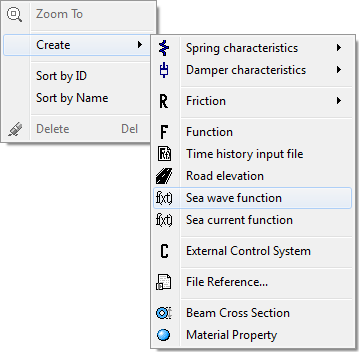
\includegraphics[trim=0 52 0 0,clip,width=0.55\textwidth]{Figures/4a-SeaWaveFunction}
\end{wrapfigure}

You create a wave function by right-clicking an empty space in the Model Manager
{\sl Objects} list, selecting \textbf{Create} and then
\textbf{Sea wave function}.
You can also access the command from the {\sl Marine} menu.
The new wave function, which is automatically selected,
is added to the list of {\sl Wave functions} maintained in the Model Manager
{\sl Objects} list.

The properties of the created wave function
\noindent\begin{minipage}{0.65\textwidth}\raggedright
are shown in the Property Editor panel.
It is similar to the property panel of general functions
\end{minipage}

\vskip-2pt\noindent (see \refSection{function-properties}{Function properties}),
except that the {\sl Argument} frame is absent.
The wave functions are always functions of spatial location and time, and the
{\sl Function Type} selection is limited to the following periodic functions:

\begin{itemize}
\item\protect\hyperlink{sine-wave}{Sine}
\item\protect\hyperlink{jonswap-sea-wave-spectrum}{JONSWAP sea wave spectrum}
\item\protect\hyperlink{user-defined-wave-spectrum}{User defined wave spectrum}
\end{itemize}

These three types of sea wave function types are described in detail below.

\clearpage

\SubSubSection{Sine}{sine-wave}

Wave functions of type {\sl Sine} are used to model regular waves, defined from
a constant amplitude $A$, angular frequency $\omega$,
and phase shift $\epsilon$.

The property panel of the {\sl Sine} wave function is shown below.

\noindent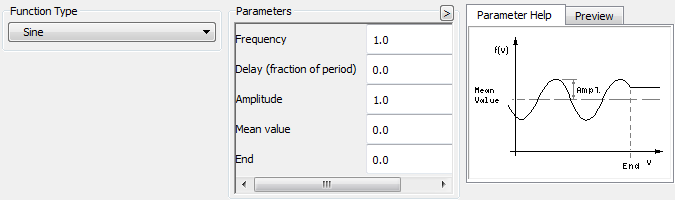
\includegraphics[width=\textwidth]{Figures/4a-SineFunction}

\Note{This property panel is the same as that of general Sine functions
  (see \refSubSection{sine}{Sine}{function-types}. Thus, the {\rm Frequency}
  and {\rm Delay} parameter values specified here are multiplied by $2\pi$
  to become the $\omega$ and $\epsilon$ parameters, respectively.
  The {\rm Mean value} and {\rm End} parameters are also not used.}

In case of infinite water depth, the wave elevation above the mean sea water
level, $h$, the horizontal and vertical water particle velocities,
$\{v_x,v_z\}$, and the horizontal and vertical water particle acceleration,
$\{a_x,a_z\}$, are given as the following functions of time, $t$,
and the spatial coordinates, $x$ and $z$,
referring to the coordinate system defined in
\refSection{coordinate-system-for-wave-kinematics}
           {Coordinate system for wave kinematics}:
%
\begin{eqnarray}
 h \;\;\;\;&=& A \sin\omega t - kx + \epsilon \\[2mm]
 \left\{\!\!\begin{array}{c} v_x \\ v_y \end{array}\!\!\right\} &=&
 \omega Ae^{kz}\left\{\begin{array}{c}
  \sin\left(\omega t - kx + \epsilon\right) \\
  \cos\left(\omega t - kx + \epsilon\right)
 \end{array}\right\} \\[2mm]
 \left\{\!\!\begin{array}{c} a_x \\ a_y \end{array}\!\!\right\} &=&
 \omega^2Ae^{kz}\left\{\begin{array}{c}
  \sin\left(\omega t - kx + \epsilon\right) \\
  \cos\left(\omega t - kx + \epsilon\right)
 \end{array}\right\}
\end{eqnarray}
%
where $k=\omega^2/g$ is the wave number
($g=\|{\bf g}\|$ being the gravity constant).

In the case of finite water depth (see bullet \TextBullet{3} in
\refSection{sea-environment}{Sea environment}), the expression for
the wave elevation is the same as above, but the wave number, $k$,
is now determined from the following nonlinear equation
%
\begin{equation}
\frac{\omega^2}{g} = k\tanh kd
\end{equation}
%
where $d$ is the average water depth.
This equation is solved for each wave component,
through Newton iterations before the time integration is started.
The water particle velocity and acceleration
are then calculated from the following expressions during the time integration:
%
\begin{eqnarray}
 \left\{\!\!\begin{array}{c} v_x \\ v_y \end{array}\!\!\right\} &=&
 \frac{\omega A}{\sinh kd}\left\{\begin{array}{c}
  \cosh\left(kz+kd\right)\sin\left(\omega t - kx + \epsilon\right) \\
  \sinh\left(kz+kd\right)\cos\left(\omega t - kx + \epsilon\right)
 \end{array}\right\} \\[2mm]
 \left\{\!\!\begin{array}{c} a_x \\ a_y \end{array}\!\!\right\} &=&
 \frac{\omega^2A}{\sinh kd}\left\{\begin{array}{c}
  \cosh\left(kz+kd\right)\sin\left(\omega t - kx + \epsilon\right) \\
  \sinh\left(kz+kd\right)\cos\left(\omega t - kx + \epsilon\right)
 \end{array}\right\}
\end{eqnarray}

\noindent{\sl\textbf{Wheeler stretching}}

\noindent The expressions above for the water particle velocity and
acceleration have a term depending on the vertical coordinate $z$
to model the exponential decay of the motion variables as we go deeper.
This term has the value 1.0 at the water surface ($z=0.0$) and then decreases
exponentially towards zero. However, above the mean water level ($0 < z \le h$),
i.e., inside a wave crest, this term will be larger than 1.0 and then give
an unreasonable high velocity and acceleration.
To avoid this, Fedem employs {\sl Wheeler stretching}
on the velocity/acceleration expressions.
That is, the $z$-coordinate is replaced a modified value $z'$, where
%
\begin{eqnarray}
z' &=& z-h \quad\quad\;\:\mbox{for infinite water depth} \\
z' &=& \frac{z-h}{d+h}\cdot d \quad\mbox{for finite water depth}
\end{eqnarray}

\begin{wrapfigure}[11]{r}{0.4\textwidth}
  \vskip-\baselineskip
  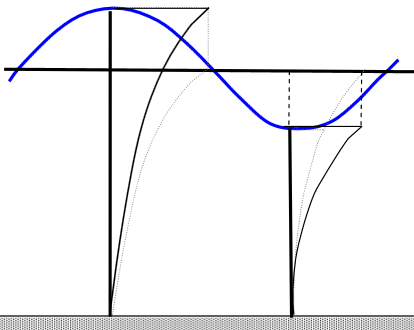
\includegraphics[trim=50 0 10 0,clip,width=0.4\textwidth]{Figures/4a-wheelerStretching}
\end{wrapfigure}

For the case of finite water depth,
the effect of this modification is illustrated in the figure to the
right. As can be seen, the magnitude is reduced inside a wave crest, but
increased below a wave trough.

Alternatively, a simple vertical stretch may be employed,
which means we use $z'=0.0$ when $z>0.0$.
To use this formulation, specify
{\tt -noWheelerStretching} in the Additional Solver Options dialog box,
{\sl Dynamics Solver} field,
see \refSection{additional-solver-options}{Additional solver options},
before the simulation is started.

\SubSubSection{JONSWAP sea wave spectrum}{jonswap-sea-wave-spectrum}

Wave functions of type {\sl JONSWAP (Joint North Sea Wave Project)
sea wave spectrum} are used to model irregular waves.
Basically, these functions consist of a sum of simple Sine wave functions,
as defined above, where the Amplitude, Frequency and Phase delay parameters
varies for each component. These parameters are calculated from a few
user-specified parameters, such that the resulting wave function
exhibits some predefined statistical properties.

The property panel of the JONSWAP sea wave function is shown below.

\noindent
\begin{picture}(344,95)
\put(0,0){\includegraphics[width=\textwidth]{\ReferenceImg/prp/wave-function-1}}
  \put(93,52){\Bullet{1}}
  \put(93,30){\Bullet{2}}
  \put(93,18){\Bullet{3}}
  \put(46,6){\Bullet{4}}
  \put(99,6){\Bullet{5}}
  \put(215,75){\Bullet{6}}
  \put(215,63){\Bullet{7}}
  \put(215,48){\Bullet{8}}
\end{picture}

\begin{bulletlist}
\item{\sl Spectral peakedness} --
  This is a non-dimensional parameter ($\gamma$) that defines the peakedness
  of the wave components. The default value is 3.3.
  If the {\sl Use DNV recommendation} toggle is enabled, $\gamma$ is calculated
  automatically from the specified significant wave height and spectral peak
  period based on the formulas given below.
\item{\sl Number of wave components} --
  Number of wave components ($n$) to use in the spectrum.
\item{\sl Number of wave directions} --
  Number of concurrent wave directions if wave spreading is desired
  (1 means unidirectional waves).
\item{\sl Spreading exp.} --
  Spreading exponent defining the sharpness of the wave spreading,
  if the number of wave directions is specified larger than 1.
\item{\sl Random seed} --
  This is a non-negative integer value that is used as random seed in
  the pseudo-random generator, which delivers a sequence of random values
  in range $[0.0,1.0]$. These random values are used to compute the phase delay
  ($\epsilon\in[0,2\pi]$) for each wave component, and the size of the frequency
  intervals ($\Delta\omega_j=\omega_j-\omega_{j-1}$) between each wave component.
\item{\sl Significant wave height} --
  This value specifies the significant wave height ($H_s$)
  from through to crest. The value is given in meters,
  or the current length dimension used.
\item{\sl Spectral peak period} --
  This value specifies the peak period ($T_p$) of the wave spectrum in seconds.
\item{\sl Period cut-off values} --
  This defines the frequency range to use in the wave spectrum
  ($\omega_0=2\pi/T_{\rm high}$ and $\omega_n=2\pi/T_{\rm low}$).
  If the {\sl Automatically calculate period cut-off values} toggle is enabled,
  the $T_{\rm low}$ and $T_{\rm high}$ values are calculated automatically based on
  the formulas below.
\end{bulletlist}

Based on the property parameters above, the amplitude, $A_j$,
for wave component $j$ with a given angular frequency $\omega_j$ is computed as
%
\begin{equation}
A_j = \sqrt{2S(\omega_j)\Delta\omega}
\end{equation}
%
where $S(\omega)$ denotes the actual wave spectrum and $\Delta\omega$
is a constant difference between successive frequencies in the spectrum.

The JONSWAP spectrum is defined as follows\footnote{
See S.~K.~Chakrabarti, {\sl Hydrodynamics of Offshore Structures}, WIT Press,
1987, pp. 105--116 and the DNV-RP-C205 {\sl Environmental conditions and
Environmental loads}, October 2011, pp. 33--34, for a full development
of the wave spectrum formulae.}:
%
\begin{equation}
S(\omega) = A_\gamma\frac{5}{16}\frac{H_s^2\omega_p^4}{\omega^5}
           \exp\left(-\frac{5}{4}\left(\frac{\omega}{\omega_p}\right)^{-4}\right)
           \gamma^Y
\end{equation}
\begin{equation*}
A_\gamma = 1 - 0.287\ln(\gamma)\;,\quad
Y = \exp\left(-\frac{1}{2}\left(\frac{\omega-\omega_p}{\sigma\omega_p}\right)^2
        \right)
\end{equation*}
%
where $H_s$ is the significant wave height,
$\omega_p=2\pi/T_p$ is the spectral peak frequency,
$\gamma$ is the peakedness parameter and $\sigma$ is a spectral shape parameter.
The latter is set equal to 0.07 for frequencies $\omega$ less than or equal to
$\omega_p$ and to 0.09 for frequencies greater than $\omega_p$.

The spectral peakedness is calculated based on recommendation in the DNV-RP-C205
(see footnote 1 below), if the the {\sl Use DNV recommendation} toggle
is enabled in the property panel (see above). This reads as follows
%
\begin{equation}
\gamma \;=\left\{\begin{array}{lll}
5 &\forall& \tau \le \frac{18}{5} \\
\exp\left(\frac{23}{5}-\frac{23}{20}\tau\right) &\forall& \frac{18}{5}<\tau<5 \\
1 &\forall& \tau > 5
\end{array}\right.
\end{equation}
%
where the parameter $\tau$ is defined as $\tau=\frac{T_p}{\sqrt{H_s}}$.

\Note{If the peakedness parameter $\gamma$ is set to 1.0,
such that $A_\gamma=\gamma^Y=1.0$, then the JONSWAP wave spectrum becomes
equal to the so-called Pierson--Moskowitz Spectrum.}

If the {\sl Automatically calculate period cut-off values} toggle is enabled
in the property panel, the highest and lowest period values are calculated
based on the peak period, $T_p$, and the peakedness parameter, $\gamma$, through
%
\begin{equation}
T_{\rm low} = T_p\left(\frac{4\tilde{m}_o^{\rm cut}}{5A_\gamma}\right)^{1/4},\quad
T_{\rm high} = T_p\left(\frac{\ln\left(A_\gamma/\tilde{m}_o^{\rm cut}\right)}{5/4}
                \right)^{1/4}
\end{equation}
%
where $A_\gamma$ is as defined above,
and the value $\tilde{m}_0^{\rm cut}$ is set to 0.0025 (i.e., 0.25\%).
See the DNV RP-C205 for further elaboration.

\SubSubSection{User defined wave spectrum}{user-defined-wave-spectrum}

Wave functions of type {\sl User defined wave spectrum} are similar to the
\protect\hyperlink{jonswap-sea-wave-spectrum}{JONSWAP sea wave spectrum}
functions, except from that the Amplitude, Frequency and Phase delay parameters
(and optionally also the wave numbers) for each wave component, now are
read from an ASCII file instead of calculating them from input parameters.

The property panel of the User defined wave spectrum function is shown below.
It contains a {\sl File/Reference} field through which the ASCII file
containing the wave spectrum is specified.

\noindent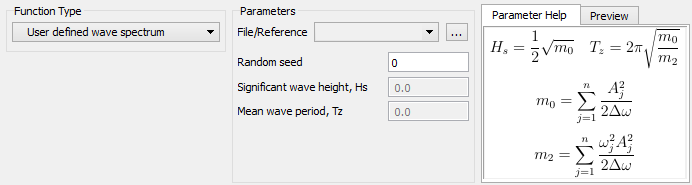
\includegraphics[width=\textwidth]{Figures/4a-WaveSpectrumFromFile}

The specified file is assumed to consist of either 2, 3 or 4 white-space
separated columns of data, with the following interpretation:

\begin{enumerate}
\item Wave amplitude [m]
\item Frequency [Hz]
\item Phase delay in fraction of the wave period [0,1]
\item Wave number ($k$) [m$^{-1}$]
\end{enumerate}

The number of columns must be specified on the first line in the file,
via the string {\tt"\#ncol <n>"} where {\tt"<n>"} is the value 2, 3 or 4.
If the first line does not contain the string {\tt\#ncol}, a two-column file
is assumed. If the file consists of either two or three columns,
the wave numbers are calculated automatically based on the gravitation constant
($g$), the angular frequency ($\omega$), and the water depth ($d$) in case for
finite depth formulation, as described above for the
\protect\hyperlink{sine-wave}{Sine} wave functions.
If the file consists of two columns only, the phase delay of each wave component
is assigned using the internal pseudo-random generator, as for the
\protect\hyperlink{jonswap-sea-wave-spectrum}{JONSWAP sea wave spectrum}
functions.

The property panel also contains two fields displaying the
{\sl Significant wave height} ($H_s$) and the {\sl Mean wave period} ($T_z$),
which are derived from the provided amplitude ($A_j$)
and frequency data ($\omega_j$) based on the formulas shown in the
{\sl Parameter Help} view tab.

\clearpage


\SubSection{Sea current functions}{sea-current-functions}

Sea current functions specify the current velocity magnitude and direction
as functions of water depth and time. The resulting current velocity vector
is superimposed to the velocity of the specified wave function, if any,
to get the overall fluid velocity on which the hydrodynamic load calculations
are based.

\Note{It is assumed that the time dependency on the current velocity is so
  weak that the water particle acceleration derived from it can be ignored.
  Thus, no acceleration-dependent hydrodynamic loads will result from the
  specified current.}

\begin{wrapfigure}[7]{r}{0.55\textwidth}
  \vskip-\baselineskip
  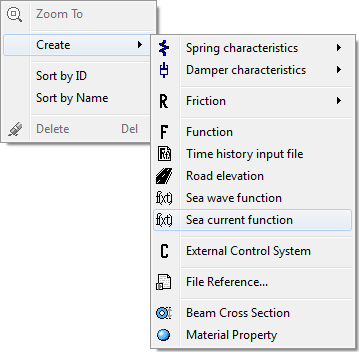
\includegraphics[trim=0 50 0 0,clip,width=0.55\textwidth]{Figures/4a-SeaCurrentFunction}
\end{wrapfigure}

You create a current function by right-clicking an empty space in the Model
Manager {\sl Objects} list, selecting \textbf{Create} and then
\textbf{Sea current function}. You can also access the command from the
{\sl Marine} menu.
The new current function, which is automatically selected,

\noindent\begin{minipage}{0.63\textwidth}\raggedright
is added to the list of {\sl Current functions} maintained in the Model Manager
{\sl Objects} list.
\end{minipage}

The properties of the created current function
\vskip0pt\noindent\begin{minipage}{0.68\textwidth}\raggedright
are shown in the Property Editor panel.
It is identical to the property panel of the general functions
(see \refSection{function-properties}{Function properties}),
\end{minipage}

\vskip-2pt\noindent except that the {\sl Argument} frame now is absent.
The current functions are functions of the vertical coordinate ($z$)
of the wave coordinate system only (see
\refSection{coordinate-system-for-wave-kinematics}
           {Coordinate system for wave kinematics}).
However, if the type is set to {\sl Math Expression},
a function of all the spatial coordinates ($x, y, z$)
referring to the wave coordinate system, and the time $t$ may be defined.


%%%%%%%%%%%%%%%%%%%%%%%%%%%%%%%%%%%%%%%%%%%%%%%%%%%%%%%%%%%%%%%%%%%%%%%%%%%%%%%%
\Section{Response amplitude operators}{response-amplitude-operators}

The goal of a vessel Response Amplitude Operator (RAO) is to express the motion
of a point on a rigid vessel floating in the sea as a function of the wave
height at the same reference point. The concept of a RAOs is associated with the
stationary sinusoidal response (or motion) of a linear system due to a
stationary sinusoidal load (wave). Due to the assumption of system linearity,
the following is true:

\clearpage
\begin{enumerate}
\item
  The response amplitude is proportional to the wave amplitude for a given wave
  period, e.g., twice the wave amplitude will give twice the response amplitude.
\item
  The response period is exactly equal to the wave period, e.g., a sinusoidal
  wave with a period of 10 seconds will cause a sinusoidal response with
  a period of 10 seconds.
\item
  The response and the wave are usually not in phase. Therefore, the extreme
  value of the wave and the response usually do not occur at the same time.
\end{enumerate}

For a reference point at the origin of the wave coordinate system (see
\refSection{coordinate-system-for-wave-kinematics}
           {Coordinate system for wave kinematics}),
the wave height for a regular wave (or for one component of an irregular wave),
is written as the following function of time $t$):
%
\begin{equation}
h = A\sin\left(\omega t + \epsilon\right)
\end{equation}
%
The associated motion response is then assumed on the form
%
\begin{equation}
\label{eq:RAO}
R = BA\sin\left(\omega t + \epsilon + \phi\right)
\end{equation}
%
where $A$ is the wave amplitude, $\omega$ is the angular frequency
and $\epsilon$ is the phase delay of the wave, whereas $B$ and $\phi$
are the relative amplitude and phase angle, respectively, of the RAO.
Tables of $B$ and $\phi$ are provided for a given vessel for each of the
six DOFs in the reference point, and for different incoming wave angles,
see \refSection{creating-raos}{Creating RAOs} below.


\SubSection{Creating RAOs}{creating-raos}

\IconTextFirst{RAO}{
  You can create an RAO in Fedem by selecting
  \textbf{Response Amplitude Operator} in the {\sl Marine} menu.
  An object of type {\sl Vessel Motion} is then created, along with six general
  functions representing the motion of the vessel in the six individual DOFs
  of the vessel's reference point. The created Vessel Motion object is
  automatically selected, such that its topology view and property panel
  (shown below) are displayed.}

\noindent
\begin{picture}(344,75)
  \put(0,0){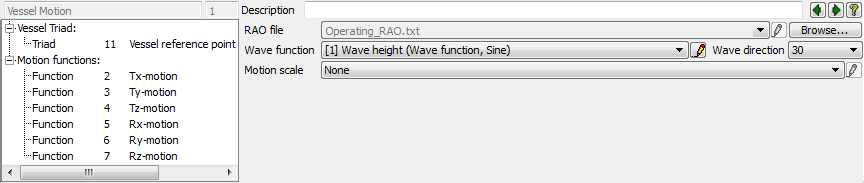
\includegraphics[width=\textwidth]{Figures/4a-RAO}}
  \put(45,50){\Bullet{1}}
  \put(70,25){\Bullet{2}}
  \put(200,55){\Bullet{3}}
  \put(210,48){\Bullet{4}}
  \put(320,48){\Bullet{5}}
  \put(200,40){\Bullet{6}}
\end{picture}

\begin{bulletlist}
\item{\sl Vessel Triad} --
  This specifies the reference point of the vessel.
  When at least one of the Motion functions is assigned as prescribed motion in
  a given Triad, that one is automatically recognized as the Vessel Triad.

\item{\sl Motion functions} --
  Here, the created six functions that represent the actual motion
  of the vessel reference point are listed:

  \begin{enumerate}
  \subitem Tx-motion -- translation in local $X$-direction
  \subitem Ty-motion -- translation in local $Y$-direction
  \subitem Tz-motion -- translation in local $Z$-direction
  \subitem Rx-motion -- rotation about local $X$-axis
  \subitem Ry-motion -- rotation about local $Y$-axis
  \subitem Rz-motion -- rotation about local $Z$-axis
  \end{enumerate}

  These functions are all on the form as given by Equation~(\ref{eq:RAO}),
  where the $A$, $\omega$ and $\epsilon$ values are taken from the selected
  {\sl Wave function}, whereas $B$ and $\phi$ are read from the {\sl RAO file.}

\item{\sl RAO file} --
  This field specifies a file containing the RAO table(s) describing the
  vessel motion as functions of wave elevation and frequency.
  Use the \textbf{Browse...} button to select the file to be used.
  See \refSection{rao-table-format}{RAO table format},
  for description of the RAO file format.

\item{\sl Wave function} --
  This field specifies the wave function defining the wave height ($A$),
  angular frequency ($\omega$) and phase delay ($\epsilon$) used by
  the motion functions. Normally, this should be the same function as specified
  as the Wave function in the Sea Environment dialog box (see
  \refSection{sea-environment}{Sea environment}), but is not necessarily so.

\item{\sl Wave direction} --
  This pull-down menu contains the list of wave direction angles that are
  specified in the selected RAO file. They define the angle (in degrees)
  between the local $X$-axis of the {\sl Vessel Triad} and the incoming
  wave direction, i.e., a zero wave direction means that the waves propagate
  in the direction of the negative local $X$-axis of the Vessel Triad
  and the value 90.0 means that the waves propagate in the direction
  of the negative $Y$-axis. A separate RAO table is associated with
  each of the direction angles in the RAO file.

\EnumNote{In addition to selecting the actual RAO table to use,
  the Wave direction angle also affects the wave kinematics
  (i.e., the water particle velocity and acceleration),
  and thereby also the hydrodynamic forces acting on the submerged part
  of the mechanism, since it is also used to define the local $X$-axis of the
  wave coordinate system, relative to the local axes of the Vessel Triad.}

\item{\sl Motion scale} --
  This field specifies a General Function to be used as a scaling on the six
  generated {\sl Motion functions} in bullet \TextBullet{2}.
  This can be used to ramp up the RAO motions in a smooth manner,
  to avoid undesired startup transients. When a function is specified here,
  six new motion functions are generated, where each one is defined as
  the product of the original motion function and the scaling function.
\end{bulletlist}

After creating the Vessel Motion object, you must manually assign the six
created motion functions as Prescribed motions to the Triad that defines the
vessel reference point. All six functions must be assigned to the same Triad.
It is also possible to leave out some of the functions, if, for instance,
some are identically zero and/or you want to study the response in 2D only.
However, if some of the functions are referred by another Triad (or Joint),
a {\sl Vessel Triad} is not identified and the RAO will not work.

If a {\sl Motion scale} function is specified after you have assigned the
original motion functions to the vessel reference triad, those functions are
automatically replaced by the scaled versions.
Moreover, if you later change the Motion scale function back to {\sl None},
the scaled motion functions are removed again and the references to the original
functions are restored. Thus, you only need to change the {\sl Motion scale}
function setting to efficiently toggle the RAO scaling on or off.


\SubSection{RAO table format}{rao-table-format}

A sample RAO file is shown below. An RAO file consists of a series of tables,
each with 14 columns of data. Each table is started by the line

{\tt Direction \textless angle\textgreater}

\noindent where \textless angle\textgreater{} is the wave direction
as discussed above (see \refSection{creating-raos}{Creating RAOs}).
Any line starting with an apostrophe (') is treated as comments,
and can be used for increased human readability.

\noindent\fbox{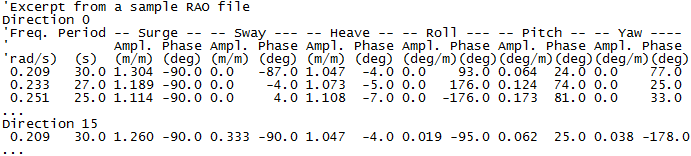
\includegraphics[width=\textwidth]{Figures/4a-RAOsample}}

The first two columns of each table list the angular {\sl frequency} and
corresponding wave {\sl period}, respectively, of the wave components.
The period value is not used, it is listed for information only. However,
it can not be omitted from the file (a dummy value of 0.0 is fine though).

The angular frequencies must be listed in increasing order within each table,
and linear interpolation is used between the two closest frequencies listed,
for actual wave components with frequencies not present in the table.
Flat extrapolation is used for values lower than the first frequency listed
in the table, or higher than the last frequency listed.

The remaining 12 columns list pairs of {\sl amplitude} scales and {\sl phase}
delays (the $B$ and $\phi$ quantities as defined through
Equation~(\ref{eq:RAO})) for the six DOFs (Surge, Sway, Heave, Roll, Pitch
and Yaw) of the vessel reference point.


%%%%%%%%%%%%%%%%%%%%%%%%%%%%%%%%%%%%%%%%%%%%%%%%%%%%%%%%%%%%%%%%%%%%%%%%%%%%%%%%
\Section{Beam string structures}{beam-string-structures}

A beam string in Fedem is an assembly of several {\sl Beams} (beam elements)
which are connected to each other in {\sl Triads} along an (initial) straight
line. A beam string is represented by a sub-assembly object of the sub-type
{\sl Beamstring} in the Fedem model
(see \refSection{sub-assemblies}{Sub-assemblies}).
It can be used to model typical one-dimensional marine structures,
such as flexible risers, anchoring lines, umbilicals, etc.


\SubSection{Import of beam strings}{import-of-beam-strings}

\IconTextFirst{riser}{\vskip-2mm
  You can create a beam string by selecting \textbf{Import Beamstring} from the
  {\sl Marine} menu. A plain dialog box through which you can select an input
  file containing the definition of the beam string and its properties then pops
  up. The format of the beam string definition file is described in
  \refSection{beam-string-file-format}{Beam string file format"} below.}

The triads and beam elements of the beam string assembly are generated from a
specified starting point, and in the opposite direction of the gravitation
vector as defined in the Sea Environment dialog box (see
\refSection{sea-environment}{Sea environment}).
Therefore, if a non-vertical beam string is desired, you have to temporarily
change the gravitation vector while performing the beam string import.


\SubSection{Beam string file format}{beam-string-file-format}

The beam string input file lists the properties of the beam structure, from the
starting (bottom) point and up. All blank lines and text lines in the file are
ignored (treated as comments) except for a limited set of keywords and part
names, as described below. The position of new-line characters is arbitrary with
in a data section of the file. Thus, you may add or remove as many new-line
characters you wish to improve readability.

The first three numerical values in the file are assumed to be the global
coordinates ($x, y, z$) of the beginning of the beam.
Then, an arbitrary number of the following data sections are assumed
(in arbitrary order):
%
\begin{center}
\vskip0.5\baselineskip
\begin{minipage}{0.9\textwidth}
\begin{verbatim}
<part name>
<Rho> <E> <G> <Do> <Di> <Dd> <Db> <Cd> <Cm> <Ca>
<L> <nel>
"<vis-file>"

Ball Joint

Free Joint
<Zpos>

Cylindric Joint
<Zpos>
\end{verbatim}
\end{minipage}
\vskip0.5\baselineskip
\end{center}
%
The interpretation of these keywords and values are as follows:
%
\begin{itemize}
\item{\tt<part name>} -- Description to be assigned to the beams (optional).
  Whether a part name is specified or not is determined based on the first
  non-space character in this line; if it is neither a digit nor any of the
  characters '.', '-' or '+' it is assumed that a part name is given.
\item{\tt<Rho>} -- Structural mass density.
\item{\tt<E>} -- Young's modulus of elasticity.
\item{\tt<G>} -- Shear modulus of elasticity.
\item{\tt<Do>} -- Outer pipe diameter.
\item{\tt<Di>} -- Inner pipe diameter.
\item{\tt<Dd>} -- Drag diameter.
\item{\tt<Db>} -- Buoyancy diameter.
\item{\tt<Cd>} -- Drag coefficient.
\item{\tt<Cm>} -- Added mass coefficient for fluid.
\item{\tt<Ca>} - Added mass coefficient for structure.
\item{\tt<L>} -- Total length of this beam segment.
\item{\tt<nel>} -- The number of beam elements this segment is divided into.
\item{\tt<vis-file>} -- Path to a visualization file describing
  the geometry to be displayed for each element of this beam segment (optional).
  Unless an absolute path is given, the path is assumed to be relative to the
  folder of the beam string input file.
\item{\tt Ball joint} -- Creates a Ball Joint at current location.
\item{\tt Free Joint} -- Creates a Free Joint with master triad at
 current location and slave triad at the given position.
\item{\tt Cylindric Joint} -- Creates a Cylindric Joint with masters at the two
  latest generated triads, and slave triad at the given position.
\item{\tt<Zpos>} --
  Global position from starting point in beam string direction.
\end{itemize}

\noindent A sample beam string input file is shown below:

\vskip\baselineskip
\noindent\fbox{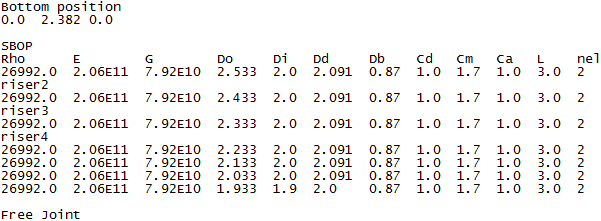
\includegraphics[width=\textwidth]{Figures/4a-RiserSample}}
\vskip\baselineskip

Each beam segment is divided into the specified number of elements of uniform
length {\tt<L>/<nel>}. A triad is created between each beam element that a beam
segment consists of. The end triad of one segment automatically becomes the
starting point of the next, or the master triad of the subsequent Joint,
if specified.

A beam cross section object
(see \refSection{beam-cross-sections}{Beam cross sections})
is generated for each beam segment and assigned the structural-
and hydrodynamic properties listed above (assuming a {\sl Pipe} cross section).
This object is referred to by each beam element of that segment such that
hydrodynamic loads (added mass and drag forces, as well as buoyancy)
can be calculated for the beam string based on these properties
(see \refSection{hydrodynamic-loads-on-beam-elements}
                {Hydrodynamic loads on beam elements}).

\clearpage


\SubSection{Beam string properties}{beam-string-properties}

The property panel of a {\sl Beamstring} object is shown below:

\noindent
\begin{picture}(344,92)
  \put(0,0){\includegraphics[width=\textwidth]{\ReferenceImg/prp/riser-1}}
  \put(40,55){\Bullet{1}}
  \put(24,41.5){\Bullet{2}}
  \put(24,31.5){\Bullet{3}}
  \put(44,21){\Bullet{4}}
  \put(130,70){\Bullet{5}}
  \put(208,70){\Bullet{6}}
  \put(332,70){\Bullet{7}}
  \put(203,37){\Bullet{8}}
  \put(285,81){\Bullet{9}}
\end{picture}

\begin{bulletlist}
\item{\sl Is internal to:} -- Currently not used.

\item{\sl Mass} --
  This field displays the total weight of the beam string structure.
  It is computed as the sum of the structural mass of the individual beam
  elements that the beam string consists of.
  Additional mass due to marine growth
  (see \refSection{marine-growth}{Marine growth}) and/or internal liquid
  (see \refSubSection{mass-from-internal-fluid}{Mass from internal fluid}
  {hydrodynamic-loads-on-beam-elements} is {\sl not} included.

\EnumTip{To get a mass distribution overview when the effects of marine growth
  and/or internal liquid is accounted for, see the mass summary in the
  \File{fedem\_solver.res} file after the Dynamics solver has been started.}

\item{\sl Length} --
  This field displays the total length of the beam string, i.e.,
  the sum of the length of each element that the beam string consists of.

\item{\sl Visualize 3D} --
  This toggle turns on and off the 3D-visualization of all beam elements
  contained in the beam string assembly.
  The {\sl Start} and {\sl Stop} fields are used to specify
  a sector of partial 3D visualization.
  They define the start and stop angles (in degrees), relative to the local
  $Y$-axis of the cross section, of the sector that is to be rendered in 3D.

\EnumNote{This Visualize 3D toggle has a tri-state value.
  In addition to the usual on 
\includegraphics[scale=0.5]{Figures/Icons/on}
  and off 
\includegraphics[scale=0.5]{Figures/Icons/off} states, it can also
  have a neither-on-nor-off 
\includegraphics[scale=0.5]{Figures/Icons/onoff}
  state, in which the corresponding on or off settings on each element are
  applied instead. This is usually the default setting for such tri-state
  toggles and indicates that the corresponding setting on the element level
  is not unique.}

\item{\sl Internal Liquid} --
  This toggle enables the calculation of additional mass due to internal liquid
  (mud) in the beam string (see \refSubSection{mass-from-internal-fluid}
  {Mass from internal fluid}{hydrodynamic-loads-on-beam-elements}).

  \begin{itemize}
  \subitem{\sl Mud density} -- Mass density of the internal liquid.
  \subitem{\sl Mud level} -- Global $Z$-coordinate of the mud level.
  \end{itemize}
  Only those beam elements having their centre of gravity below the
  {\sl Mud level} are assumed to be filled with mud.

\item{\sl Structural Damping} --
  Use these fields to apply common mass- and stiffness-proportional damping
  parameters to all beam string members.

\item{Scaling of Dynamic Properties} --
  Use these fields to apply common stiffness and mass scaling to all beams
  in the beam string.

\EnumNote{If any of the structural damping and stiffness/mass scaling fields are
  blank, it means that the beam elements of the beam string do not have a
  common value for that property. This typically occurs after you edit the
  Beam property directly.}

\item{Position and Orientation} --
  These fields can be used to adjust the global position of the beam string
  assembly after it has been imported.
  They work as those of the {\sl Origin} property tab, see
  \refSection{origin-property}{Origin property}.
  An assembly can be moved freely until it is attached to ground,
  or connected to other mechanism objects.

\item{\sl Subassembly model file} --
  A separate model file may be assigned to the beam string assembly by using the
  \textbf{Browse...} button. In that case, all the beams, triads and properties
  of this beam string are stored in the specified file when the model is saved.
  It is then possible to reuse this beam string in another model
  by importing it into an existing model
  (see \refSection{importing-sub-assemblies}{Importing sub-assemblies}).
  If the {\sl Subassembly model file} field is empty, the elements of the beam
  string are stored in the main model file together with the rest of the model.
\end{bulletlist}


\SubSection{Mooring line generation}{mooring-line-generation}

\vskip23mm
\IconTextFirst{beam}{\vspace*{-22mm}
  A mooring line is a 1D structure with very low bending stiffness that can be
  modeled as a chain of beam elements, and where the shape between the two
  end points are mostly determined by the own weight of the structure.
  Fedem offers a tool for easy generation of such structures in a equilibrated
  modeling configuration.}
  \vskip-10mm

\begin{wrapfigure}[8]{r}{0.37\textwidth}
  \vskip-1.2\baselineskip
  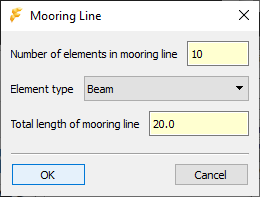
\includegraphics[width=0.37\textwidth]{Figures/Dialogs/4-MooringLine}
\end{wrapfigure}

\noindent To create a mooring line, select two Triads in \newline
the {\sl Modeler} view or from the {\sl Objects} list in \newline
the Model Manager panel, and select \newline
\textbf{Mooring Line...} from the {\sl Marine} menu.
The dialog box shown to the right then appears.

Here, you can specify the number of elements and the total length of the mooring
line to be generated. You may also change the element type to {\sl Generic Part}
instead of {\sl Beam}, or to any other two-noded user-defined element you may
have. Then select \textbf{OK} to generate the elements.
If the two selected Triads are member of a common sub-assembly, the generated
elements and Triads will become members of that sub-assembly also.


%%%%%%%%%%%%%%%%%%%%%%%%%%%%%%%%%%%%%%%%%%%%%%%%%%%%%%%%%%%%%%%%%%%%%%%%%%%%%%%%
\Section{Space frame structures}{space-frame-structures}

A space frame in Fedem is an assembly of several {\sl Beams}
which are connected to each other in {\sl Triads}.
An arbitrary number of beams may be connected at each Triad.
Thus, it becomes a full FE representation of the structure on the system level.
A space frame is represented in the Fedem model by a Sub-assembly object of the
sub-type {\sl Jacket} (see \refSection{sub-assemblies}{Sub-assemblies}.
A Jacket is a model of a bottom-fixed off-shore structure, which typically are
used as foundation for wind turbines and oil exploration platforms.
The beam members of a Jacket structure may therefore be assigned properties for
hydrodynamic load calculation (added mass and drag coefficients, etc.,
see \refSection{hydrodynamic-loads-on-beam-elements}
               {Hydrodynamic loads on beam elements}).


\SubSection{Import of space frames}{import-of-space-frames}

\IconTextFirst{jacket}{
  You can import a space frame by selecting \textbf{Import Spaceframe...}
  from the {\sl Marine} menu. The dialog box shown below then pops up.}

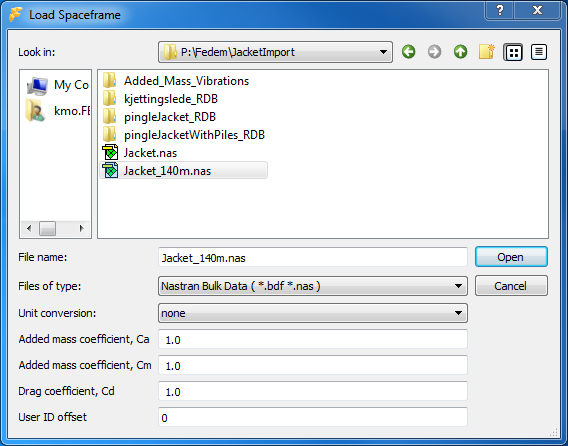
\includegraphics[width=0.7\textwidth]{Figures/4a-LoadSpaceframe}

It has similar fields for selecting an FE model file as the Load Part dialog box
(see \refSection{creating-parts-by-file-import}{Creating parts by file import}).
Note that only beam, spring and point mass elements will be read by this import.
Any existing shell and solid elements present in the imported FE model file will
be ignored. A complete list of the ignored elements (if any) are provided in the
Output List view (see \refSection{output-list}{Output List}).

The Load Spaceframe dialog box also has fields for specification of added mass
and drag coefficients ({\sl Ca}, {\sl Cm} and {\sl Cd}). These will be the
default values that are applied to all beam members of the imported space frame.

By default, the Beam and Triad objects that are created during the import will
receive as user ID the external ID stored in the FE model file for the
corresponding beam element and FE node. However, a constant offset value may be
specified in the {\sl User ID offset} field in the dialog box.


\SubSection{Space frame properties}{space-frame-properties}

The property panel of a {\sl Jacket} or space frame object is shown below:

\noindent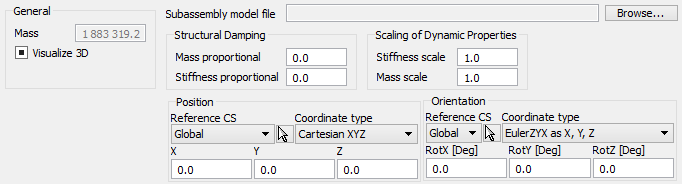
\includegraphics[width=\textwidth]{Figures/4a-JacketProperty}

It is similar to the property panel of the {\sl Beamstring} object
(see \refSection{beam-string-properties}{Beam string properties}),
except that the {\sl Is internal to:} and the {\sl Length} fields are absent
(irrelevant for space frame structures), as well as the {\sl Start} and
{\sl Stop} angle fields for 3D visualization.
The {\sl Internal Liquid} fields are also absent although the beam elements of
a space frame may be liquid-filled.
Instead, the mass density of the internal liquid and the liquid level are
assumed identical to the {\sl Water density} and the {\sl Mean sea level},
respectively, as defined in the Sea Environment dialog box
(see \refSection{sea-environment}{Sea environment}).
Whether a beam is to be considered liquid-filled or not is in this case toggled
by specifying a non-zero diameter of the internal liquid ({\sl Di})
in the cross section referred by the beam
(see \refSubSection{hydrodynamic-properties}{Hydrodynamic properties}
{hydrodynamic-loads-on-beam-elements}.
See also \refSubSection{mass-from-internal-fluid}{Mass from internal fluid}
{hydrodynamic-loads-on-beam-elements} for more details on calculation
of additional mass from internal liquid.

The data fields present in the {\sl Jacket} property panel has a similar
interpretation as the corresponding fields found in the {\sl Beamstring}
property panel. We therefore refer to
\refSection{beam-string-properties}{Beam string properties}
for a detailed description of these fields.


%%%%%%%%%%%%%%%%%%%%%%%%%%%%%%%%%%%%%%%%%%%%%%%%%%%%%%%%%%%%%%%%%%%%%%%%%%%%%%%%
\Section{Soil Pile structures}{soil-pile-structures}

A soil pile in Fedem is similar to a beam string
(see \refSection{beam-string-structures}{Beam string structures})
in the sense that it consists of several {\sl Beams} connected to each other in
{\sl Triads} along a straight line. In addition, the soil pile contains several
{\sl Free joints} with nonlinear spring characteristics that model the soil
interaction for the pile
(see figure on \hyperref[soil-springs]{page \thechapter-25}). A soil pile
is represented by a Sub-assembly object of the sub-type {\sl Soil Pile}
in the Fedem model (see \refSection{sub-assemblies}{Sub-assemblies}).


\SubSection{Import of soil piles}{import-of-soil-piles}

\IconTextFirst{soilpile}{
  You can import a soil pile by selecting \textbf{Import Soil Pile...}
  from the \emph{Marine} menu. The dialog box shown below then pops up,
  in which you can select the file that contains the soil pile definition.
  See \refSection{soil-pile-file-format}{Soil pile file format}
  for a description of the soil pile definition file format.}

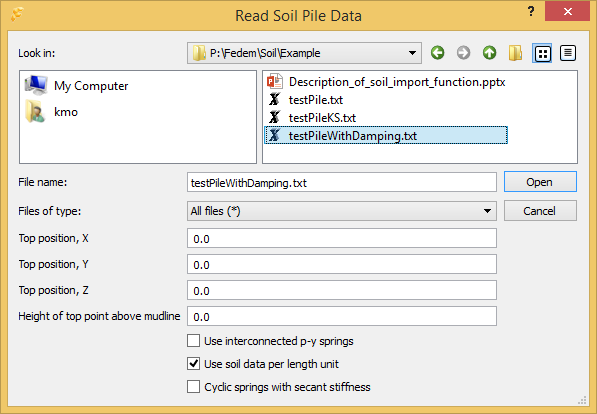
\includegraphics[width=0.8\textwidth]{Figures/Dialogs/4-ImportSoilPile}

The Read Soil Pile Data dialog box has three fields ({\sl Top position, X},
{\sl Top position, Y} and {\sl Top position, Z}) for specification of the
global position of the top of the pile. The beams representing the pile are then
generated from this top point, and in the direction of the gravitation vector.

The {\sl Height of top point above mudline} field (HT) defines where the mudline
is located, relative to the top point
(see figure on \hyperref[soil-springs]{page \thechapter-25}).
The location of the soil springs along the pile are then specified relative to
this mudline level.

The Read Soil Pile Data dialog box has in addition three toggles that affect the
generated Free Joint and spring objects of the pile:

\begin{itemize}
\item{\sl Use interconnected p-y springs} --
  Enables that the soil springs work in the radial direction with respect to
  the pile axis. This is achieved by setting the {\sl Translation} spring
  inter-connectivity to {\sl Cylindrical Z} for the generated Free joints,
  see \refSubSection{advanced-joint-properties}{Advanced joint properties}
  {joint-properties}.

\item{\sl Use soil data per length unit} --
  If enabled, the soil spring data is treated as stiffness/force per length unit
  and is scaled by the segment length of each beam to obtain the effective
  Force/Stiffness to be applied in the discrete Free joints,
  see \refSection{soil-pile-file-format}{Soil pile file format} below.
  This is the default setting. If you have discrete soil pile data instead,
  remember to switch off this toggle.

\item{\sl Cyclic springs with secant stiffness} --
  Enables a secant stiffness behavior when the soil is unloaded,
  see \refSection{secant-stiffness-on-unloading}{Secant stiffness on unloading}
  below.
\end{itemize}


\SubSection{Soil pile file format}{soil-pile-file-format}

The soil pile input file lists the properties of the pile, from the starting
point at (or above) mudline and downwards. All blank lines and text in the file
are ignored (treated as comments) except for a limited set of keywords
as described in the following.

A sample input file is shown below. It consists of the following sections
which may be repeated arbitrarily, except for that the sections {\tt q-z}
and {\tt dq-z} can only appear once and at the end of the file:

\begin{center}
\vskip\baselineskip
\begin{minipage}{0.8\textwidth}
\begin{verbatim}
Pipe <rho> <E> <G> <OD> <ID>

Depth <Z> [<nel>]
<sd_type>
[Symmetric]
<x0> <f0>
<x1> <f1>
...
\end{verbatim}
\end{minipage}
\end{center}

\clearpage\noindent
\begin{minipage}{0.5\textwidth}\raggedright
\begin{itemize}
\item{\tt Pipe} --
  Specifies the structural properties of the pile (mass density,
  Young's and shear moduli, outer and inner pipe diameter)
  valid from current Dept level until the next Pipe keyword is encountered.

\item{\tt Depth} --
  Specifies the depth below mudline ({\tt Z}) of the next soil spring,
  and optionally the number of beam elements ({\tt nel}) from the previous
  soil spring, \newline or start of the pile.

\item{\tt sd\_type} --
  Heading defining the soil spring/damper type.
  The following eight keywords are recognized:

  \begin{namelist}{\tt dq-z}
  \item[\tt p-y] Normal spring
  \item[\tt dp-y] Normal damper
  \item[\tt t-z] Tangential spring
  \item[\tt dt-z] Tangential damper
  \item[\tt r-z] Rotational spring \newline (about pile axis)
  \item[\tt dr-z] Rotational damper \newline (about pile axis)
  \item[\tt q-z] Axial spring at the \newline bottom end of the pile
  \item[\tt dq-z] Axial damper at the bottom end of the pile
  \end{namelist}
\end{itemize}
\end{minipage}\begin{minipage}{0.5\textwidth}
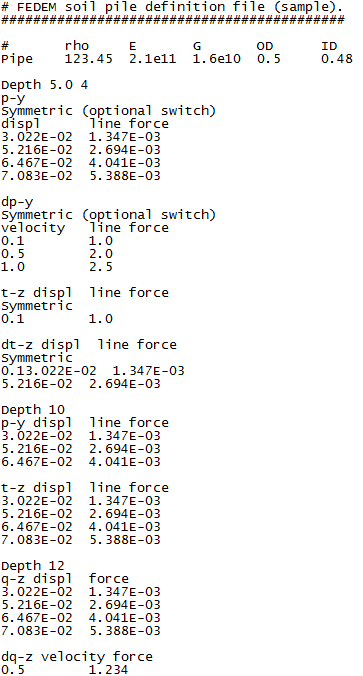
\includegraphics[width=1.05\textwidth]{Figures/4a-PileSample}
\end{minipage}

\begin{itemize}
\item{\tt Symmetric} --
  Optional keyword indicating that the subsequent spring/damper properties are
  symmetric for positive and negative deflections/velocities, such that only
  the force values for positive deflection/velocity need to be listed.

\item{$x_i$, $f_i$} --
  Points on the force-deflection curve for the nonlinear soil spring
  (or force-velocity curve for dampers). The points must be listed for
  increasing values of deflection/velocity ($x_i$).
\end{itemize}

\phantomsection\label{soil-springs}{}
\noindent\begin{minipage}{0.6\textwidth}\raggedright
The force values ($f_i$) are given as line force intensity along the pile [N/m].
The total force for a certain deflection in a spring at depth level $D_j$
is thus $F_j=f_jL_j$, for $j=1\ldots n-1$, where (see figure to the right):
%
\begin{eqnarray*}
L_1 &=& \frac{1}{2}(D_1 + D_2) \\
L_j &=& \frac{1}{2}(D_{j+1} + D_{j-1})\;,\quad 1<j<n-1 \\
L_{n-1} &=& D_n -\frac{1}{2}(D_{n-1} + D_{n-2})
\end{eqnarray*}

The bottom soil spring/damper is not subjected to this length scaling.
The force values ($f_i$) for these springs are therefore \newline
given in directly Newtons [N].\vskip5\baselineskip\mbox{}
\end{minipage}\begin{minipage}{0.4\textwidth}
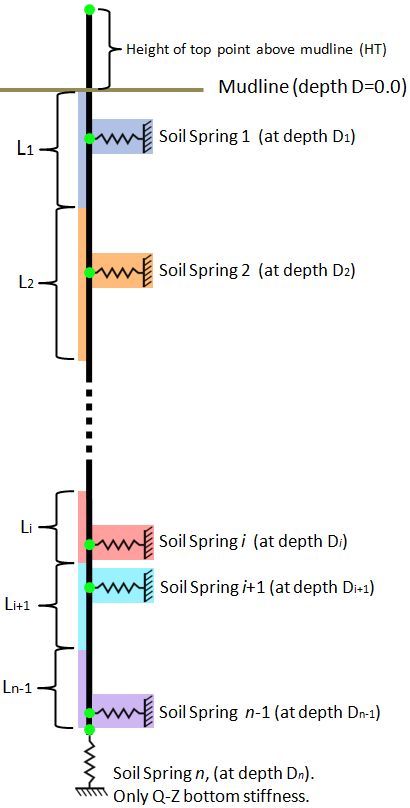
\includegraphics[width=\textwidth]{Figures/4a-SoilPile}
\end{minipage}


\SubSection{Secant stiffness on unloading}{secant-stiffness-on-unloading}

\begin{wrapfigure}[12]{r}{0.6\textwidth}
  \vskip-1.1\baselineskip
  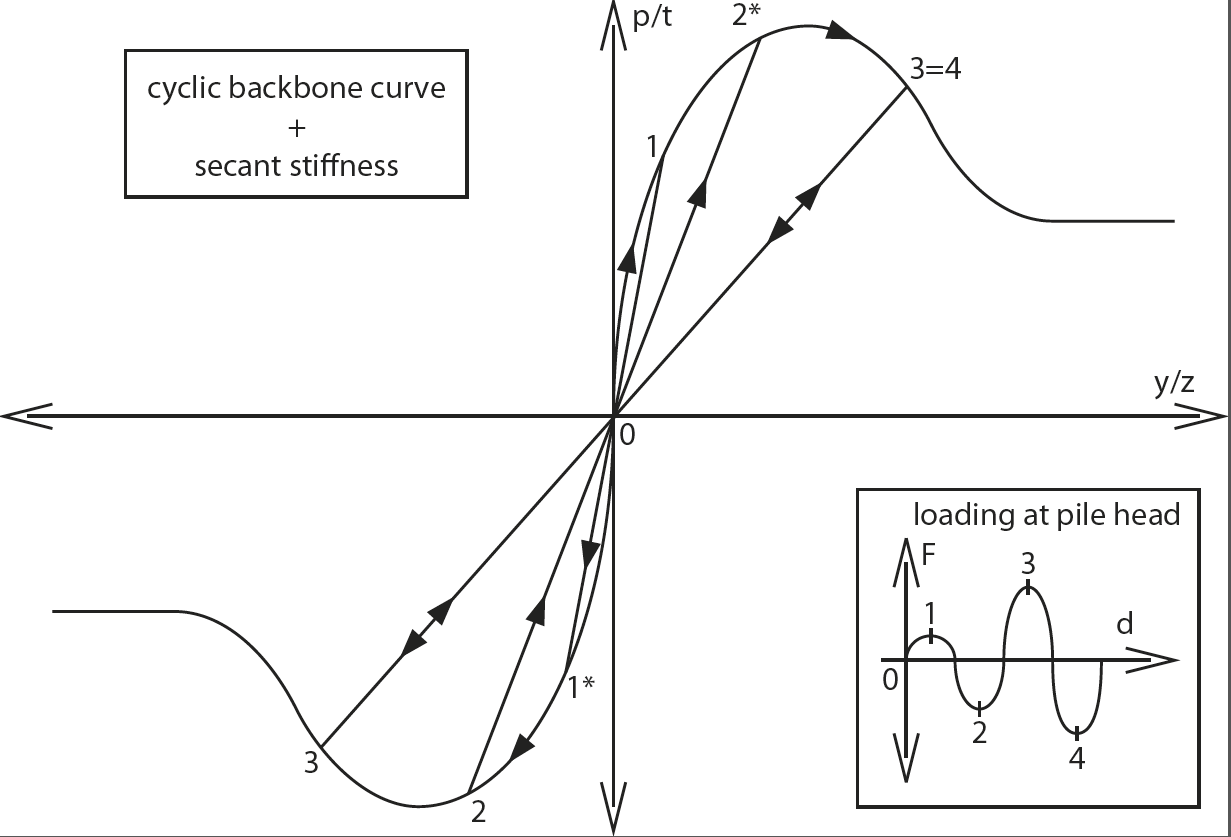
\includegraphics[trim=0 4 3 0,clip,width=0.6\textwidth]{Figures/4a-SoilSpring}
\end{wrapfigure}

The soil springs are normally regarded as hyperelastic, i.e., when a spring is
unloaded (the deflection decreases) the force follows the same
force-displacement curve as when the deflection increases (and similar for the
damping force versus velocity). However, when the {\sl Cyclic springs with
secant stiffness} toggle is enabled in the Read Soil Pile Data dialog box
(see \refSection{import-of-soil-piles}{Import of soil piles}),
the normal springs (p-y curves) are interpreted as cyclic back-bone curves with
a secant stiffness (see figure to the right).
The resulting secant stiffness is a function of the largest deflection
experienced so far during the loading history.


\SubSection{Soil pile property}{soil-pile-property}

The property panel of a {\sl Soil pile} object is shown below:

\noindent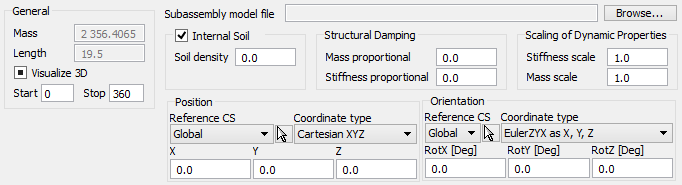
\includegraphics[width=\textwidth]{Figures/4a-SoilProperty}

It is similar to the property panel of the {\sl Beamstring} object
(see \refSection{beam-string-properties}{Beam string properties}), except that
the {\sl Is internal to:} field is absent (irrelevant for soil pile structures).
The {\sl Internal Liquid} toggle and fields are replaced by a similar toggle for
{\sl Internal Soil} and a {\sl Soil density} field.
If internal soil is enabled, the entire soil pile is assumed filled with soil
and it is therefore no soil level field in this property panel.
The effect of the internal soil is similar as the internal liquid in beam
strings and jacket members, see
\refSubSection{mass-from-internal-fluid}{Mass from internal fluid}
{hydrodynamic-loads-on-beam-elements}.

The other data fields present in the {\sl Soil Pile} property panel has a
similar interpretation as the corresponding fields found in the {\sl Beamstring}
property panel. We therefore refer to
\refSection{beam-string-properties}{Beam string properties} for a detailed
description of these fields.

\Note{Soil piles are also subjected to Buoyancy based on the specified water
  density, if they are located under the mean sea level as defined in the
  Sea Environment dialog (see \refSection{sea-environment}{Sea environment}
  and \refSubSection{hydrodynamic-properties}{Hydrodynamic properties}
  {hydrodynamic-loads-on-beam-elements}.}


%%%%%%%%%%%%%%%%%%%%%%%%%%%%%%%%%%%%%%%%%%%%%%%%%%%%%%%%%%%%%%%%%%%%%%%%%%%%%%%%
\Section{Hydrodynamic load calculations}{hydrodynamic-load-calculations}

\SubSection{Buoyancy of 3D volumes}{buoyancy-of-3d-volumes}

Buoyancy forces (and associated load correction stiffness) may be included for
any {\sl Generic Part}, if the part is assigned a geometry description file in
the {\sl Visualization} field in the part property
(see \refSubSection{part-tab}{Part tab}{part-properties}), and the
{\sl Perform buoyancy calculations} toggle in the
\protect\hyperlink{hydrodynamics-tab}{\sl Hydrodynamics tab} is enabled.
The geometry description file has to define a closed volume that represents the
total displaced fluid body when the part is submerged, and can be either on the
VRML-format or the Fedem Technology Cad format (\File{.ftc},
see \refSection{ftc-format}{FTC format}).

The buoyancy force is computed from that part of the volume that is below the
specified sea water level surface and is applied in the opposite direction of
the gravitation vector. In the buoyancy calculation, the water surface is
assumed as the plane that contains the point $\frac{s_0}{\|{\bf g}\|}{\bf g}$,
where $s_0$ denotes the current sea water level,
and $\bf g$ is the gravitation vector.
The normal vector of the sea water plane is equal to the opposite of the
gravitation vector. The sea water level is either a constant
(given by the {\sl Mean sea level} parameter in the Sea Environment dialog box,
see \refSection{sea-environment}{Sea environment}) or a function of space and
time, when a {\sl Wave function} is specified in the Sea Environment dialog box.
In the latter case, the current sea level is taken as the wave elevation
evaluated at the local origin of the Generic Part in question.

\Note{When using a wave function, it is assumed that the cross section between
  the buoyant volume and the water surface is sufficiently small compared with
  the dominant wave length, as the change in water surface normal is not
  accounted for.}


\SubSection{Hydrodynamic loads on beam elements}
           {hydrodynamic-loads-on-beam-elements}

Beam elements in Fedem, that is, the basic elements of {\sl Beamstring},
{\sl Jacket} and {\sl Soil Pile} components, may be subjected to hydrodynamic
loads, based on the defined wave kinematics as described in
\refSection{wave-and-current-functions}{Wave and current functions}
and some additional hydrodynamic property parameters,
see \refSection{hydrodynamic-properties}{Hydrodynamic properties} below.
This provides a simplified modeling of the actual loads acting on beam
structures partly or fully submerged in sea water.
All hydrodynamic load calculations are performed assuming a circular
outer cross section shape of the beams.


\SubSubSection{Hydrodynamic properties}{hydrodynamic-properties}

The property panel of the {\sl Beam cross section} objects is described in
\refSection{beam-cross-sections}{Beam cross sections}.
In addition to the {\sl Structural} parameters discussed there,
it has a set of hydrodynamic property parameters grouped in a separate tab,
as shown below:

\noindent
\begin{picture}(325,95)
  \put(5,0){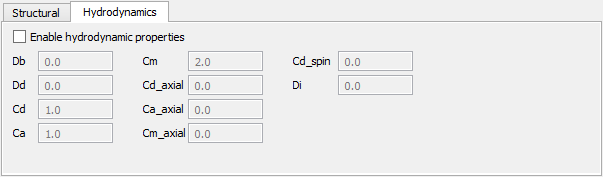
\includegraphics[width=0.95\textwidth]{Figures/4a-hydro}}
  \put(-3,71){\Bullet{1}}
  \put(-3,58){\Bullet{2}}
  \put(-3,45){\Bullet{3}}
  \put(-3,32){\Bullet{4}}
  \put(-3,19){\Bullet{5}}
  \put(67,58){\Bullet{6}}
  \put(67,45){\Bullet{7}}
  \put(67,32){\Bullet{8}}
  \put(67,19){\Bullet{9}}
  \put(148,58){\BBullet{10}}
  \put(148,45){\BBullet{11}}
\end{picture}

\begin{bulletlist}
\item{\sl Enable hydrodynamic properties} --
  Hydrodynamic loads are only calculated for beams referring to cross sections
  for which this toggle enabled, and that are at least partly below the defined
  sea surface.
\item{\sl Db} -- Effective buoyancy diameter,
  see \protect\hyperlink{buoyancy-of-beams}{\sl"Buoyancy of beams"} below.
\item{\sl Dd} -- Effective drag diameter,
  see \protect\hyperlink{drag-and-added-mass}{\sl"Drag and added mass"} below.
\item{\sl Cd} -- Drag coefficient (in normal direction of the beam).
\item{\sl Ca} -- Added mass coefficient associated with structure motion.
\item{\sl Cm} -- Added mass coefficient associated with water particle motion.
\item{\sl Cd,axial} -- Drag coefficient in axial direction of the beam.
\item{\sl Ca,axial} -- Added mass coefficient associated with structure motion
  in axial direction of the beam.
\item{\sl Ca,axial} -- Added mass coefficient associated with water particle
  motion in axial direction of the beam
\item{\sl Cd,spin} -- Drag coefficient for relative torsional motion.
\item{\sl Di} -- Diameter of internal fluid (or soil) body,
used for calculation of additional mass,
see \protect\hyperlink{mass-from-internal-fluid}{\sl"Mass from internal fluid"}
below.
\end{bulletlist}

\Caution{The {\rm Db} and {\rm Di} parameters in the Hydrodynamics tab are also
  used for beam elements in soil piles in order to compute buoyancy and mass of
  internal soil, if enabled
  (see \refSection{soil-pile-property}{Soil pile property}).
  All the other fields in this tab are ignored for such elements.}

\Note{Buoyancy forces are calculated for beam elements in soil pile objects,
  based on the specified sea water density, and not the soil density.
  If such buoyancy is not desired, remember to set the buoyancy diameter
  ({\rm Db}) to zero, or adjust the structural mass density of the beam cross
  section object used. Buoyancy (and mass of internal soil) is included only if
  {\rm Enable hydrodynamic properties} is checked.}

\SubSubSection{Buoyancy of beams}{buoyancy-of-beams}

The buoyancy force on a beam element is computed as
%
\begin{equation}
F_b = \rho_w g \frac{\pi D_b^2}{4}L
\end{equation}
%
where $\rho_w$ is the specified mass density of the sea water
(see \refSection{sea-environment}{Sea environment}) and $L$ is the length of the
submerged part of the beam element. This buoyancy force is distributed equally
on the two triads connected to the beam, but for a partly submerged beam the
triad that is below the water surface receives a larger portion, and the total
force is then reduced depending on how much of the beam is above the surface.

\SubSubSection{Mass from internal fluid}{mass-from-internal-fluid}

When the {\sl Di} field in the {\sl Hydrodynamics} tab is non-zero (see bullet
\begin{picture}(8,8)
\put(4.2,4){\circle*{10}}\put(0,2){\color{white}\tt\footnotesize11}
\end{picture}
in \protect\hyperlink{hydrodynamic-properties}{\sl"Hydrodynamic properties"}
above), additional mass is assigned to the beam elements using this
cross section property. If the value is positive, the additional mass is
included both as inertia forces and as a static gravity load.
If it is negative, only inertia forces are included.

In either case, the additional mass is included by modifying the
structural mass density as follows:
%
\begin{equation}
\rho_b' = \rho_s + \rho_i\frac{\pi D_i^2}{4A_s}
\end{equation}
%
where $\rho_s$ and $\rho_i$ are the mass densities of the structural material
and the internal liquid, respectively, and $A_s$ is the net structural cross
section area of the beam.

\SubSubSection{Drag and added mass}{drag-and-added-mass}

Forces due to drag and added mass on a beam element are in Fedem computed based
on the Morison equation\footnote{
See, e.g., S. K. Chakrabarti, {\sl Hydrodynamics of Offshore Structures},
WIT Press, 1987, pp. 169--194, for an elaboration.}.
This is a simplified load model valid only for slender beams with circular outer
cross sections. For a completely submerged beam element, the drag and added mass
forces are given as, respectively
%
\begin{eqnarray}
\label{eq:drag}
F_d &=& \rho_w \frac{D_d}{2} L C_d (u-u_w)|u-u_w| \\
\label{eq:added-mass}
F_a &=& \rho_w \frac{\pi D_d^2}{4} L (C_a\dot{u} - C_m\dot{u}_w)
\end{eqnarray}
%
where $u$ and $u_w$ denote the structure and water particle velocities,
respectively. The forces are calculated in the two normal directions of the
beam element, and also in the tangential direction if axial drag and added mass
coefficients are provided.

\Note{For beam elements subjected to marine growth
  (see \refSection{marine-growth}{Marine growth}),
  the user-defined drag diameter {\rm Dd} is modified to account for this, i.e.,
  the actual value used in the above equations is $D_d+2t_{mg}$, where $t_{mg}$
  is the specified thickness of the marine growth layer.
  Thus, marine growth results in increased drag and added mass,
  in addition to the extra static weight.}

The drag- and added mass forces are computed individually at each end point
since they also depend on the current structure- and fluid motion at that point.
For a partly submerged beam element, the length $L$ is reduced according to how
much is below the sea surface. The force at the surface intersection point is in
that case eccentricity-transformed onto the end that is above the water.
Mass- and damping matrix contributions are also computed, based on a
differentiation of the Equations~(\ref{eq:drag}) and~(\ref{eq:added-mass}),
respectively.
